\documentclass[12pt]{ctexart}
\usepackage{amsmath}
\usepackage{unicode-math}
\usepackage{graphicx}
\usepackage{fancyhdr}
\usepackage{tikz}
\usetikzlibrary{calc}
\usepackage{pgfplots}
\pgfplotsset{compat=1.18}
\usepackage[hidelinks]{hyperref}
\usepackage{cite}
\title{Learning \LaTeX}
\author{zhao}
\date{\today}
\pagestyle{fancy}
\lhead{\author{zhao}}
\chead{\today}
\rhead{Zhao\_yue2021@bupt.edu.cn}
\lfoot{}
\cfoot{\thepage}
\rfoot{}
\renewcommand{\headrulewidth}{0.4pt}
\renewcommand{\headwidth}{\textwidth}
\renewcommand{\footrulewidth}{0pt}
\setlength{\headheight}{15pt}

\begin{document}
\maketitle
\tableofcontents
\section{Preparation}
\subsection{Hello, Beijing}
北京 is the capital of China.
\subsubsection{Hello Dongcheng District}
\paragraph{Tian'anmen Square}
is in the center of Beijing.
\subparagraph{Chairman Mao}
is in the center of 天安门广场。
\subsection{Hello 江苏}
\paragraph{南京大学} is one of the best university in 江苏。

\section{Formula}
\subsection{difference between some method to create Formula}
Einstein's $E=mc^2$.
\[E=mc^2.\]
\begin{equation}
    E=mc^2
\end{equation}
\subsection{make several continuous character to be a superscript or a subscript}
\[z=r\cdot e^{2\pi i}.\]
\subsection{square-root and fraction}
$\sqrt{x}$, $\frac{1}{2}$.
\[\sqrt{x},\]
\[\sqrt[2]{3}\]
$\sqrt[4]{3}$
\[\frac{1}{2}.\]
\subsection{other operators}
\[\pm\;\times\;\div\;\cdot\;\cap\;\cup\;\wedge\;\vee\;\geq\;\leq\;\neq\;\approx\;\equiv\]
\[\int\quad\iint\quad\iiint\quad\iiiint\quad\idotsint\]
\[\oint\quad\oiint\quad\oiiint\]
\[\odot\quad\otimes\quad\oplus\quad\bigodot\quad\bigotimes\quad\bigoplus\]
\[\oiint_\Sigma f(x,y)\mathrm{d}x\mathrm{d}y\]
\[\oiint\limits_\Sigma f(x,y)\mathrm{d}x\mathrm{d}y\]
\[(f\ast g)=\int_{-\infty}^{\infty} f(\tau)g(t-\tau)\mathrm{d}\tau\]
\[(f\ast g)=\int\limits_{-\infty}^{\infty} f(\tau)g(t-\tau)\mathrm{d}\tau\]
\[\hat{x},\tilde{x},\bar{x},\overbrace{abcdefg},\underbrace{abcdefg},\vec{x},\overrightarrow{AB},\underrightarrow{ABCD},\]
\[2NaHCO_3\triangleq Na_2CO_3+CO_2\uparrow+H_2O\uparrow\]
\[NaHCO_3\overset{\text{高温}}{\longrightarrow}Na_2CO_3+CO_2\uparrow+H_2O\uparrow\]
\[\binom{n}{k}\]
\[\angle,\triangle\]%\square
\subsection{long-formula}
\begin{multline}
    x=a+b+c+{}\\
    d+e+f+g
\end{multline}
\[\begin{aligned}
    x={}&a+b+c+{}\\
    &d+e+f+g
\end{aligned}\]
\begin{gather}
    a=b+c+d\\
    x=y+z
\end{gather}
\begin{align}
    a&=b+c+d\\
    x&=y+z
\end{align}
\subsection{piecewise-function}
\[
    y=\begin{cases}
        -x,\quad x\leq0\\
        x,\quad x>0
    \end{cases}
\]
\section{Graphics and Tables}
\subsection{Graphic}
\subsubsection{Include a graph}
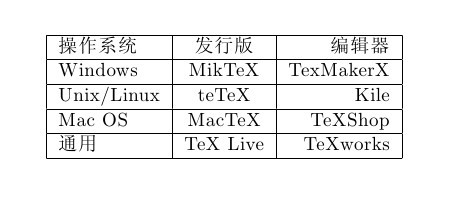
\includegraphics[width=.8\textwidth]{a.jpg}
\begin{figure}[htbp]
    \centering
    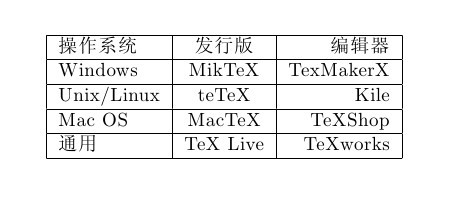
\includegraphics[width=.8\textwidth]{a.jpg}
    \caption{here is a graph}
    \label{fig:first graph}
\end{figure}
\subsubsection{Draw a graph}
\begin{tikzpicture}[scale=1]
    \draw[->] (-3,0) -- (3,0) node[below] {$x$};
    \draw[->] (0,-0.5) -- (0,5) node[left] {$y$};
    \draw[domain=-2:2,smooth,variable=\x,blue] plot ({\x},{(\x)^2});
    \draw[domain=-0.5:1.5,smooth,variable=\x,red] plot ({\x},{(\x)^3});
\end{tikzpicture}

\begin{tikzpicture}[scale=1]
    \draw[->] (-pi,0) -- (pi,0) node[below] {$x$};
    \draw[->] (0,-2) -- (0,2) node[left] {$y$};
    \draw[domain=-pi:pi,smooth,variable=\x,red] plot ({\x},{sin(\x)});
    \draw[domain=-pi:pi,smooth,variable=\x,green] plot ({\x},{sin(\x r)});
\end{tikzpicture}

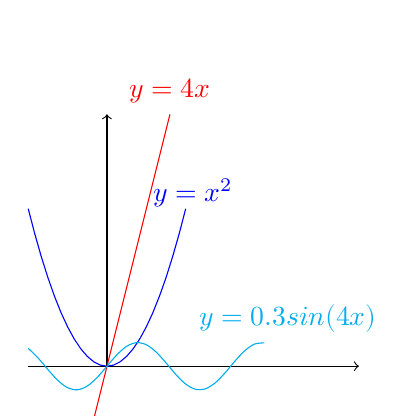
\begin{tikzpicture}[scale=1]
    \draw[<->](3.2,0)--(0,0)--(0,3.2);
    \draw(0,0)--(-1,0);
    \draw[red,domain=-0.2:0.8] plot(\x,4*\x) node at (0.8,3.5){$y=4x$};
    \draw[blue,domain=-1:1] plot(\x,2*\x*\x) node at (1.1,2.2){$y=x^2$};
    \draw[cyan,domain=-1:2,smooth] plot(\x,{0.3*sin(4*\x r)}) node at (2.3,0.6){$y=0.3sin(4x)$};
\end{tikzpicture}

\begin{tikzpicture}[scale=1]
    \begin{axis}
    \addplot[color=red]{exp(x)};
    \end{axis}
\end{tikzpicture}

%Here ends the furst plot
\hskip 5pt
%Here begins the 3d plot

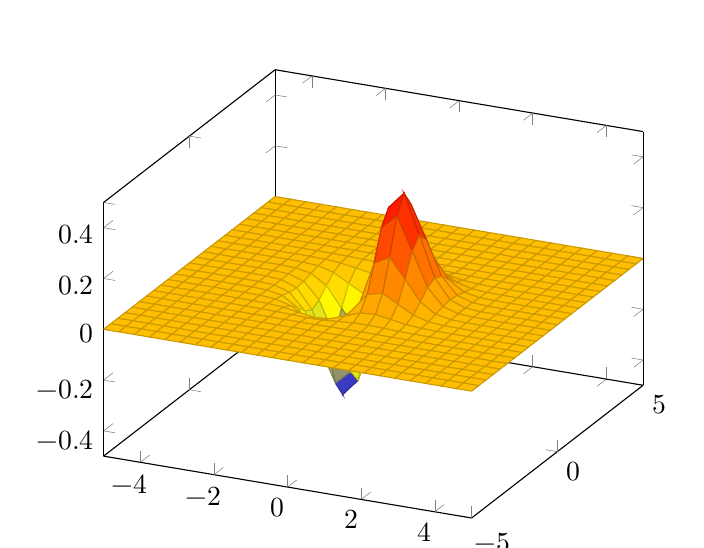
\begin{tikzpicture}[scale=1]
    \begin{axis}
    \addplot3[surf]
    {exp(-x^2-y^2)*x};
    \end{axis}
\end{tikzpicture}
\subsection{Table}
\begin{tabular}{|l|c|r|}
    \hline
    操作系统&发行版&编辑器\\
    \hline
    Windows&MikTeX&TexMakerX\\
    \hline
    Unix/Linux&teTeX&Kile\\
    \hline
    Mac OS&MacTeX&TeXworks\\
    \hline
\end{tabular}
\section{Citation}
Here is an example of how to cite someone's article: cite author\_year\textsuperscript{\cite{author_2021}}
change a line failed.

change a line sucessed.
\bibliographystyle{plain}
\bibliography{references}
\end{document}